There are primarily two forms of computer logic (Sequential and
Combinational). Traditional in electronic computers, sequential logic
requires the use of memory elements, which are not available on
quantum computers. However, for algorithms that do require extensive
use of memory, we will create mixed signal digital-quantum circuits,
which can contain memory elements, while also making use of quantum
computation.  Combinational logic on the other hand does not require
memory elements, and simply propagates input values into output
responses. 

\begin{wrapfigure}{R}{0.5\textwidth}
  \begin{center}
    \begin{tabular}{|c|c||c|c|}
      \hline
      a & b & sum & carry-out \\
      \hline 
      0&0&0&0 \\
      0&1&1&0 \\
      1&0&1&0 \\
      1&1&0&1 \\
      \hline
    \end{tabular}
  \end{center}
\end{wrapfigure}
A primary goal of this project is to refine a tool that Micah Thornton
has already constructed which can handle the synthesis of quantum
designs given a verilog specification has already been developed.  
Verilog is a computer-aided-circuit design description language,
meaning it is used to specify the functionality of circuits before
they are fabricated.  

The diagram below represents how the tool works when provided a purely
combinational specification of a simple single half-adder -- an
electronic circuit that adds two bits together, the 
truth table for this circuit is given above.  By using the quantum
synthesis tool we were able to extract the transfer matrix for this
logical operation and convert it into a quantum circuit
description.  This is a very small example, but it illustrates the
power of the tool, that performed this conversion automatically. 
\begin{center}
  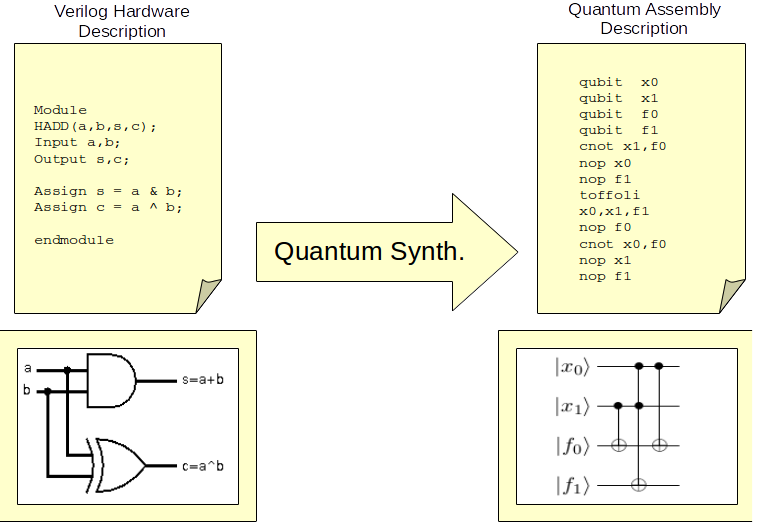
\includegraphics[scale=0.55]{QuantumSynthesis.png}
\end{center}
Within this project, we will upgrade this tool
so that it may automatically synthesize verilog descriptions of
numerical methods into their equivalent quantum forms.  With this
tool, we may then implement target numerical methods in computational
logic and automatically convert these into their quantum computing
equivalent.  Once these have been created, we will use existing
quantum simulators to test these algorithms and evaluate their promise
in quantum computing. 

